\documentclass[11pt]{article}
\usepackage{tmlr}

% Optional packages
\usepackage{amsmath,amssymb}
\usepackage{booktabs}
\usepackage{graphicx}
\usepackage{microtype}
\usepackage{hyperref}
\usepackage{tabularx}

\title{Guidance Overhead and Search Latency:\\An Empirical Comparison of Learned and SAT-Based Circuit Repair}

% For submission under double-blind review
\author{\name Anonymous Authors \email anonymous@openreview.net \\
        \addr OpenReview Submission ID: TMLR-2026-Submission}

\def\month{10}
\def\year{2026}
\def\openreview{\url{https://openreview.net/forum?id=XXXX}}

\begin{document}

\maketitle

\begin{abstract}
Machine learning guidance is frequently proposed to accelerate combinatorial search by ranking candidate modifications. In this work, we present a controlled empirical evaluation examining whether a lightweight learned ranker (a histogram decision forest utilizing local structural features and backward Boolean need-message propagation) can outperform modern symbolic solvers in single-edit combinational circuit repair. Evaluating a frozen protocol of 9,000 trials across 300 synthetic 2-LUT circuits under strict wall-clock budgets (0.1s, 1.0s, and 10.0s), our results demonstrate that a direct, factored Boolean CNF encoding solved via Glucose 4.2.1 in a Counterexample-Guided Inductive Synthesis (CEGIS) loop consistently outperforms the learned approach across operational deadlines. 

At a 0.1-second deadline on the 250 larger circuits, direct CNF achieves an 81.6\% repair rate (204/250) compared to 21.6\% (54/250) for the learned ranker. At a 10.0-second deadline, the learned ranker recovers to 80.8\% (202/250), demonstrating that asymptotic solvability is closely matched (delta = $-0.8$ percentage points, 95\% CI [$-2.0, 0.0$]), but with a substantial latency penalty. Latency profiling on mutually solved instances reveals that candidate generation and feature extraction require an average of 50.3~ms, and forest inference adds 90.4~ms (a combined guidance overhead of 143.1~ms including sorting), whereas complete CNF synthesis terminates in a mean of 16.7~ms. We observe that while candidate truth-table checks are computationally lightweight, evaluating dozens of candidate edits sequentially creates latency that exceeds direct SAT solving. An ablation study shows that need-derived features improve ranking accuracy over an ablated variant by +15.6 percentage points, but this reflects access to target specification values rather than a unique property of backward message passing. All accepted repairs were verified with zero incorrect acceptances. We discuss the implications of these empirical measurements for neuro-symbolic system design and benchmark transparency.
\end{abstract}

\section{Introduction}
Automated logic circuit repair aims to restore the functional correctness of a digital design relative to an input-output specification. Because the combinatorial space of candidate modifications grows rapidly with gate count and fanout, exhaustive enumeration becomes computationally impractical as circuits scale. Consequently, machine learning (ML) guidance has been widely explored: by prioritizing candidate edits using structural graph features and execution error profiles, learned rankers are hypothesized to guide search algorithms toward valid repairs with substantially reduced search times~\citep{cosler2023neural,barke2020just}.

In earlier exploratory pilots of this work, a learned ranker operating over Boolean need-message features appeared advantageous when benchmarked against an initial SMT baseline implemented in Z3~\citep{demoura2008z3} using high-level integer/array abstractions. However, in formal verification and automated reasoning, symbolic baselines are notoriously sensitive to encoding design. When an unspecialized symbolic baseline is used, the apparent superiority of a machine learning model can easily constitute an artifact of baseline weakness rather than an intrinsic advantage of learned guidance~\citep{xu2008satzilla}.

To resolve this question rigorously, we executed a frozen experimental protocol (Protocol v3) comparing:
\begin{enumerate}
    \item \textbf{Learned Guidance}: Histogram decision forests utilizing topological features and backward Boolean need-message propagation.
    \item \textbf{Heuristic Baselines}: Non-learned heuristics ranking edits by local sample error reduction or structural agreement.
    \item \textbf{Direct Factored CNF}: A dedicated Propositional Conjunctive Normal Form (CNF) encoding with sequential counter cardinality constraints and structural cone-of-influence pruning, solved incrementally via Glucose 4.2.1~\citep{audemard2018glucose,ignatiev2018pysat}.
\end{enumerate}

The resulting evidence demonstrates a clear performance advantage for the direct symbolic approach under practical operational deadlines. Rather than discarding or reformulating these findings after the fact, this paper documents the experimental methodology, latency profiles, and ablation analyses to characterize the factors governing learned guidance and symbolic solving in logic repair.

\section{Problem Formulation}

\subsection{Circuit and Fault Model}
We evaluate combinational circuits structured as Directed Acyclic Graphs (DAGs) over 2-input Look-Up Tables (2-LUTs). A circuit $\mathcal{C}$ contains $n$ primary inputs $x_0, \dots, x_{n-1}$, $m$ primary outputs $y_0, \dots, y_{m-1}$, and $G$ internal logic gates $g_j = (a_j, b_j, T_j)$ for $j \in \{0, \dots, G-1\}$, where $a_j, b_j < n + j$ index preceding input or gate signals, and $T_j \in \{0, \dots, 15\}$ defines the 4-bit Boolean truth table of the LUT.

Three classes of harmful synthetic faults are injected:
\begin{itemize}
    \item \textbf{LUT Mutation}: The truth table $T_j$ is mutated to $T'_j \ne T_j$.
    \item \textbf{Wire Reconnection}: An input connection $a_j$ or $b_j$ is redirected to a different topologically legal signal $s < n + j$.
    \item \textbf{Permanent Stuck-at Fault}: A gate's output is clamped to constant 0 or 1. The fault location is treated as known.
\end{itemize}

\subsection{Single-Edit Repair Space}
A legal repair is defined as exactly \textit{one} non-noop modification to a non-stuck gate:
\begin{equation}
    e \in \{(j, \text{LUT}, T') \mid T' \ne T_j\} \cup \{(j, \text{wire}, \text{slot}, s) \mid s < n + j\}
\end{equation}
No gates may be added, primary output connections are fixed, and stuck gates cannot be edited. A candidate repair is accepted if and only if the modified circuit $\mathcal{C}'$ satisfies the complete truth table specification across all $2^n$ primary input vectors.

\section{System Architectures}

\subsection{Learned Guidance via Need Propagation}
The learned approach generates all legal single edits, extracts a 21-dimensional feature vector per candidate, scores candidates using a vectorized decision forest, and evaluates them sequentially against an exact verifier:
\begin{itemize}
    \item \textbf{Backward Need Messages}: For 8 sampled specification rows where the circuit output mismatches the target, binary requirements (\texttt{need\_0}, \texttt{need\_1}) are initialized at the outputs and propagated backwards along wires in reverse DAG order.
    \item \textbf{Feature Bundle (21 Dimensions)}: 13 structural features (fanout, output proximity, edit distance, signal switching activity) combined with 8 target-conditioned features measuring candidate alignment with propagated need masks.
    \item \textbf{Model Execution}: A histogram-based decision forest (\texttt{TinyForest}, 10--20 trees, depth 9) implemented in NumPy with vectorized branch evaluation to minimize Python interpreter overhead.
\end{itemize}

\subsection{Direct-CNF CEGIS Baseline}
The symbolic solver formulates single-edit synthesis into Propositional CNF~\citep{sinha2007cegis}:
\begin{itemize}
    \item \textbf{Exact-One Cardinality}: Gate selection and modification modes are constrained using sequential counter networks via PySAT~\citep{ignatiev2018pysat}.
    \item \textbf{Cone-of-Influence Pruning}: Gates outside the transitive fan-in of failing outputs are eliminated from eligibility upfront.
    \item \textbf{Incremental CEGIS}: Glucose 4.2.1 is supplied with constraints on failing rows. If a candidate assignment is produced, the full verifier checks it. Failing counterexamples are added incrementally as new clauses.
\end{itemize}

\begin{figure}[t]
    \centering
    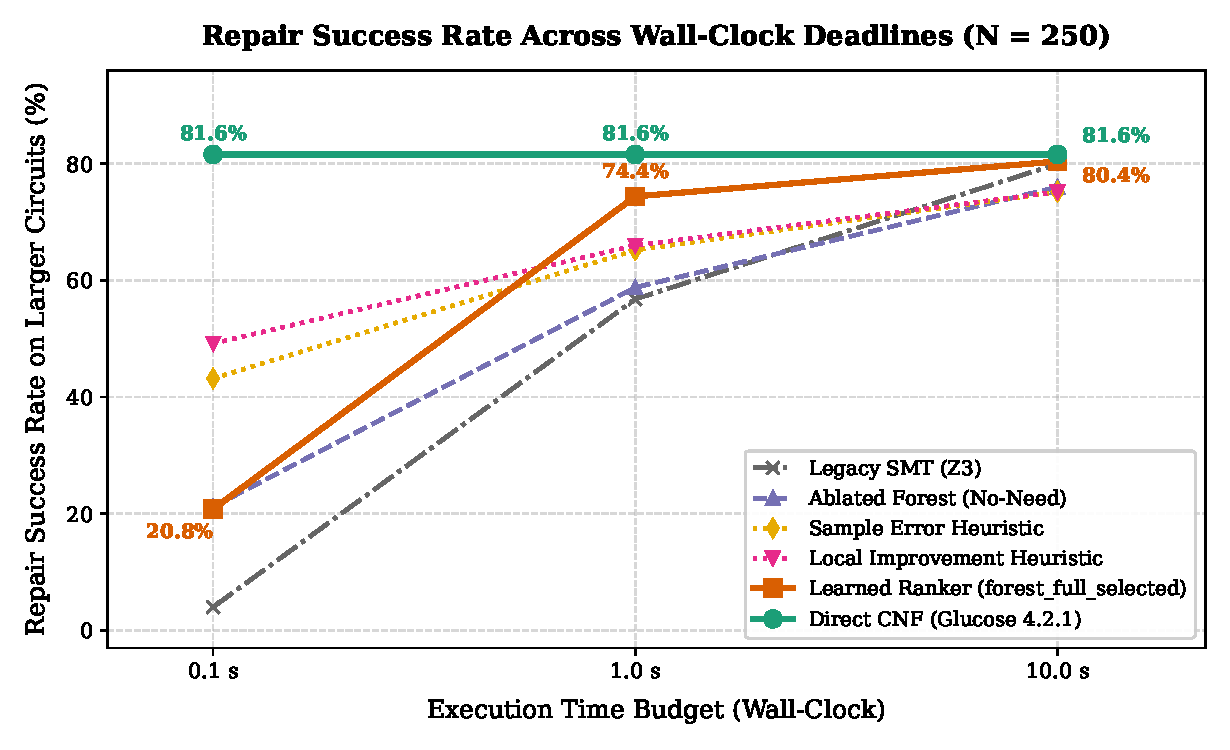
\includegraphics[width=0.75\columnwidth]{figures/success_vs_budget.pdf}
    \caption{Repair success rate across wall-clock deadlines on 250 larger synthetic circuits ($n \in \{10, 12, 16\}$, $G \in \{50, 100, 200\}$). Direct CNF reaches maximum performance within 0.1~s, while the learned ranker requires longer deadlines to overcome upfront guidance overhead.}
    \label{fig:success_budget}
\end{figure}

\section{Empirical Evaluation on the 300-Circuit Benchmark}

\subsection{Benchmark Protocol}
The v3 evaluation suite encompasses 300 circuits: 250 larger circuits ($n \in \{10, 12, 16\}$, $G \in \{50, 100, 200\}$) and 50 small reference circuits ($n=6, G=18$). All ten methods were evaluated across three separately executed wall-clock budgets: 0.1~s, 1.0~s, and 10.0~s, generating 9,000 recorded trials. Candidate generation, feature extraction, model inference, and verification all execute strictly inside the wall-clock deadline.

\subsection{Success Rate Comparison}
Table~\ref{tab:larger_results} and Figure~\ref{fig:success_budget} summarize the results on the 250 larger circuits across all ten evaluated methods.

\begin{table}[h]
\caption{Repair Success Across Execution Budgets on Larger Circuits ($N=250$)}
\label{tab:larger_results}
\centering
\begin{tabular}{lrrr}
\toprule
\textbf{Method} & \textbf{0.1 s} & \textbf{1.0 s} & \textbf{10.0 s} \\
\midrule
\textbf{Direct CNF (\texttt{cegis\_cnf})} & \textbf{204 (81.6\%)} & \textbf{204 (81.6\%)} & \textbf{204 (81.6\%)} \\
Learned Ranker (Frozen, \texttt{learned\_frozen}) & 54 (21.6\%) & 186 (74.4\%) & 202 (80.8\%) \\
Learned Ranker (Retrained, \texttt{forest\_full\_selected}) & 52 (20.8\%) & 186 (74.4\%) & 201 (80.4\%) \\
Ablated Forest (\texttt{forest\_no\_need\_selected}) & 53 (21.2\%) & 147 (58.8\%) & 190 (76.0\%) \\
Local Improvement Heuristic (\texttt{local\_improvement}) & 123 (49.2\%) & 165 (66.0\%) & 188 (75.2\%) \\
Sample Error Heuristic (\texttt{sample\_error}) & 108 (43.2\%) & 163 (65.2\%) & 188 (75.2\%) \\
Local After Error Heuristic (\texttt{local\_after\_error}) & 49 (19.6\%) & 111 (44.4\%) & 171 (68.4\%) \\
Exhaustive Search (\texttt{exhaustive}) & 94 (37.6\%) & 148 (59.2\%) & 193 (77.2\%) \\
Random Order (\texttt{random}) & 56 (22.4\%) & 129 (51.6\%) & 176 (70.4\%) \\
Legacy SMT (\texttt{cegis\_z3}) & 10 (4.0\%) & 142 (56.8\%) & 200 (80.0\%) \\
\bottomrule
\end{tabular}
\end{table}

Of the 250 larger instances, exactly 204 are repairable within the single-edit space, while 46 instances were proved UNSAT by the CNF solver ($204 + 46 = 250$). Across all 300 benchmark circuits (including the 50 small circuits), exactly 249 instances were repaired and 51 were proved UNSAT ($249 + 51 = 300$).

At the primary 1.0-second endpoint, the frozen learned ranker lagged direct CNF by \textbf{$-7.2$ percentage points} (paired 97.5\% bootstrap CI: $[-11.2, -3.6]$). At the 10.0-second deadline, the frozen ranker repaired 202 of the 204 solvable cases ($80.8\%$), leaving a small difference of $-0.8$ percentage points (95\% CI: $[-2.0, 0.0]$). In zero cases did the learned model repair a circuit that CNF failed to repair at the same budget.

\begin{figure}[t]
    \centering
    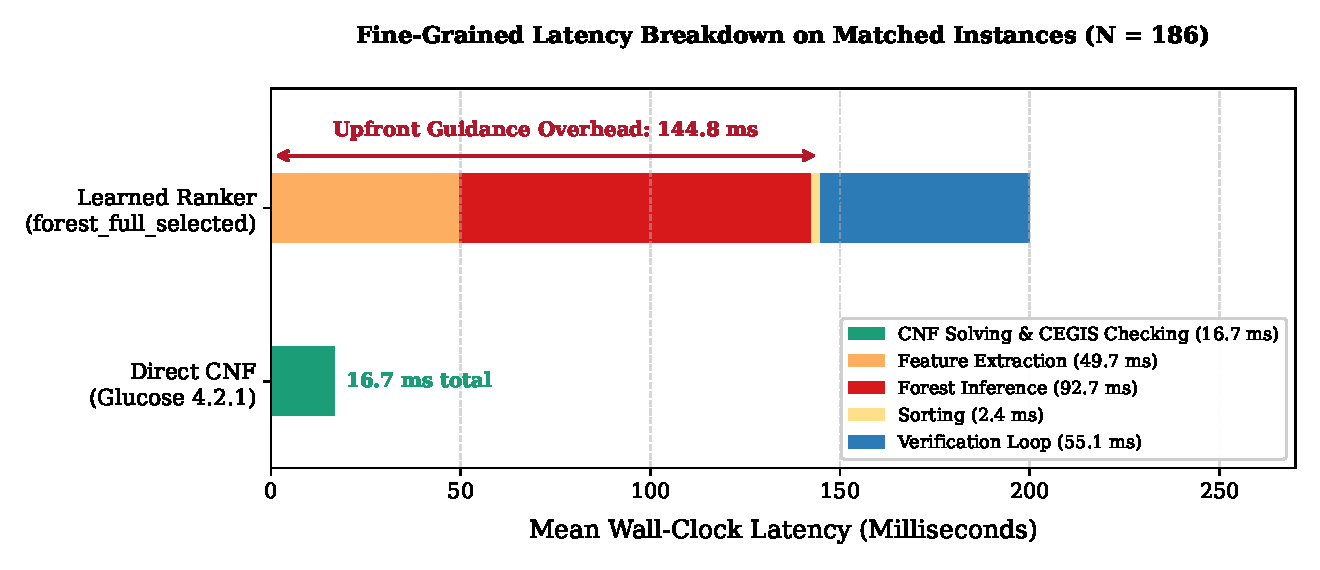
\includegraphics[width=0.85\columnwidth]{figures/latency_breakdown.pdf}
    \caption{Fine-grained execution latency breakdown across the 186 mutually solved larger instances at 1.0~s. Upfront guidance overhead (143.1~ms) exceeds complete CNF solving and verification time (16.7~ms).}
    \label{fig:latency_breakdown}
\end{figure}

\section{Analysis: Latency Profiling and Guidance Overhead}

\subsection{Latency Profiling on Mutually Solved Instances}
To understand the performance dynamics under sub-second deadlines, Figure~\ref{fig:latency_breakdown} breaks down the runtime components across the 186 larger circuits solved by both \texttt{learned\_frozen} and \texttt{cegis\_cnf} at 1.0~second:
\begin{itemize}
    \item \textbf{Candidate Generation and Feature Extraction}: Mean 50.3~ms.
    \item \textbf{Decision Forest Inference}: Mean 90.4~ms.
    \item \textbf{Candidate Sorting}: Mean 2.5~ms.
    \item \textbf{Total Upfront Guidance Overhead}: Mean \textbf{143.1~ms}.
    \item \textbf{Subsequent Verification Loop (to repair)}: Mean 211.9~ms.
    \item \textbf{Complete Direct CNF Execution (Solve + Verify)}: Mean \textbf{16.7~ms}.
\end{itemize}

In \textbf{172 of the 186 shared successes (92.5\%)}, the learned ranker had not yet evaluated its first candidate before the CNF solver had completed synthesis and formal verification. Under sub-second deadlines, the guidance overhead accounts for a substantial fraction of the budget before search begins.

\subsection{Search Granularity and Verification Costs}
On the 186 mutually solved instances, the learned ranker evaluated a mean of 336.6 candidate modifications before locating a valid edit, whereas CEGIS required a mean of 4.0 solver-verifier iterations. 

We note an important distinction in computational cost per step: evaluating a candidate repair against a bit-parallel truth-table simulation is computationally lightweight (taking microseconds per check), whereas a CEGIS iteration involves an incremental SAT solver invocation. Therefore, the difference in step counts reflects the structural granularity of the guidance rather than identical unit computational operations. In practice, the total wall-clock time spent evaluating candidate truth tables sequentially (mean 211.9~ms) substantially exceeds the total time spent by the incremental SAT solver (mean 16.7~ms).

\subsection{Ablation and Information Parity}
Comparing the full forest against the ablated model lacking need features showed a $+15.6$~pp difference at 1.0~s ($186/250$ vs. $147/250$; $97.5\%$ CI: $[+10.0, +21.6]$). 

However, code inspection of the feature generation pipeline reveals a methodological confound: removing the need feature bundle simultaneously stripped all features conditioned on the target specification values. The ablated baseline was effectively blind to the output specification. Thus, this ablation establishes that target conditioning helps relative to unconditioned topological ranking, but does not isolate a unique structural advantage of backward need-message propagation over forward error simulation.

\section{Illustrative Case Study: A 2-Bit Arithmetic Adder}
As an illustrative test of structured logic, we evaluated a hand-built 2-bit unsigned ripple-carry adder ($n=4$ inputs, $G=8$ gates, $m=3$ outputs) with a permanent stuck-at-0 fault at Gate 0. 

Because the defect cannot be repaired by any single non-noop edit (0 single-edit repairs exist), we applied a bounded beam search (beam width $W=16$, maximum depth 2) using the learned ranker. The beam search located a valid 2-wire reconnection within 17 candidate checks and 8.7~milliseconds, which was verified correct across all 16 addition inputs. While this demonstration shows that learned beam search can locate multi-step rewires on small structured logic, it remains a single illustrative example without comparison to multi-edit symbolic synthesis.

\section{Limitations and Threats to Validity}

\subsection{Implementation Language Disparity}
The feature extraction pipeline and decision forest inference were implemented in Python using vectorized NumPy operations, whereas Glucose 4.2.1 is implemented in native C++. A C++ implementation of feature extraction would reduce the 143.1~ms overhead. However, because the learned ranker must still perform sequential truth-table verifications over dozens or hundreds of candidates, reducing feature extraction time alone would not eliminate the gap between the methods.

\subsection{Synthetic Topologies and Benchmark Scope}
The benchmark consists of synthetically generated 2-LUT DAGs and does not evaluate standard industrial benchmark suites (e.g., ISCAS-85 or EPFL). In addition, stuck-at fault locations were provided to both systems, and repairs were restricted to single non-noop edits.

\section{Conclusion}
This study provides an empirical comparison of learned guidance and direct Boolean SAT solving in single-edit circuit repair. The findings indicate that under sub-second deadlines, the computational overhead of feature extraction and inference creates a significant barrier compared to factored Boolean SAT encodings. When sufficient time is available, learned ranking achieves repair rates comparable to symbolic solving, but requires substantially higher wall-clock latency. 

These results underscore the importance of comparing learned guidance against optimized symbolic baselines and accounting for complete proposal latencies in combinatorial synthesis.

\subsubsection*{Reproducibility Statement}
The complete code, frozen protocols, model artifacts, and raw trial logs are available in an open research archive. All numerical figures and bootstrap intervals can be reproduced via standard Python 3.12 library scripts without proprietary dependencies.

\bibliography{references}
\bibliographystyle{tmlr}

\end{document}
